Para realizar el test, como se mencionó, se setea en el flag frio el valor uno para testear con la cache en frio y luego en cero para testear en caliente.
Se procesan 51 imágenes $lena32.bmp$ desde la resolución 424x424 con el id: 1 (539KB) aumentando de 16x16 hasta la resolución 1224x1224 con el id: 51 (4.5MB). Cada imagen se corre 100 veces y a cada muestra, que serán los tics de reloj totales para procesar la imagen, se la divide por el tamaño de la imagen, y se toma el promedio muestral intercuartil y el desvío estandar sobre la poda realizada.

\begin{figure}[h]
  \begin{center}
	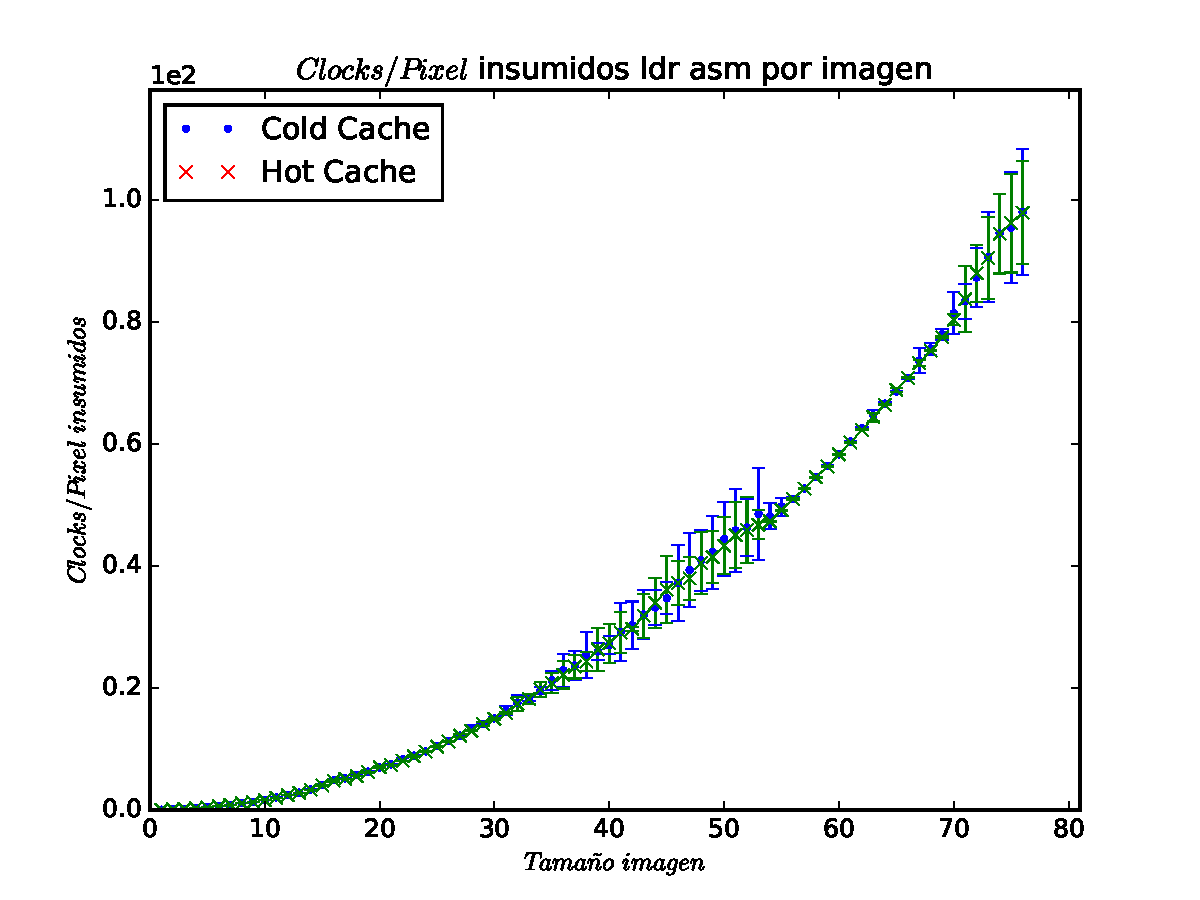
\includegraphics[scale=0.5]{ldrasmHotVsCold.pdf}
  \end{center}
\end{figure}

\begin{figure}[h]
  \begin{center}
	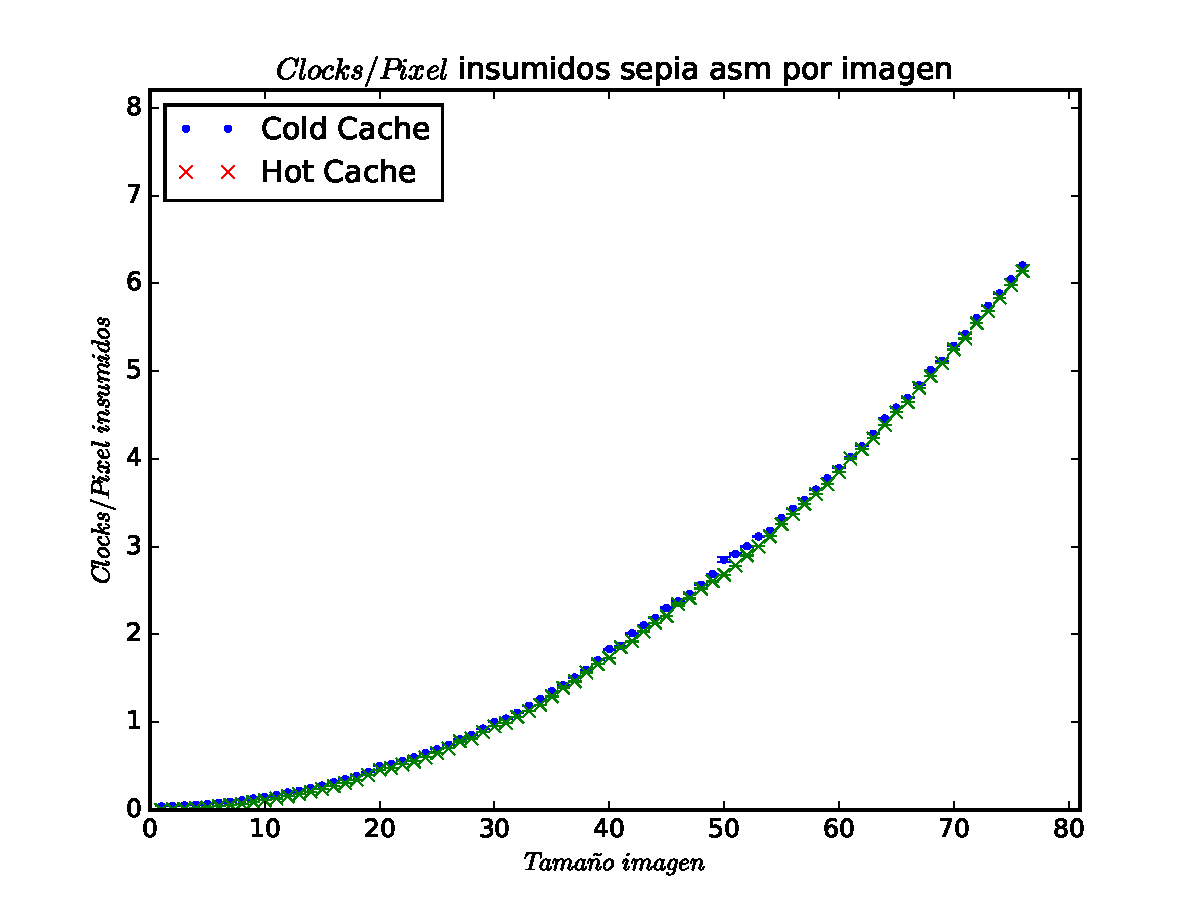
\includegraphics[scale=0.5]{sepiaasmHotVsCold.pdf}
  \end{center}
\end{figure}

\begin{figure}[h]
  \begin{center}
	\includegraphics[scale=0.5]{cropflipasmHotVsCold.pdf}
  \end{center}
\end{figure}

Podemos observar que salvo en $ldr$ todos los demás filtros mantienen el test de caché caliente por debajo del test en frio. Aunque por muy poca diferenca (menor al 0,2)
En principio esto es algo que tiene sentido. Una linea de caché tiene 64 bytes, por lo cual como ya hemos mencionado solo entrarn 16 pixeles en una linea. \\

Para el test en caliente las imágenes de menos de 3MB estarán completamente en memoria caché y tendremos 16/16 $hits$ = 100 $\%$ de $hits$ por linea. Es decir que nunca habrá necesidad de ir a buscar a memoria RAM pixeles de la imágen.\\ 
Para el test en frio lo que sucederá no es muy diferente. \\

Al no estar la imagen previamente en caché, el primer acceso será un $miss$ pero como el controlador caché utiliza el principio de localidad espacial traera a caché un bloque contiguo a una linea de la caché. Con lo cual los 15 accesos siguientes serán $hits$ por tendremos 15/16 $hits$ = 93,75 $\%$ de $hits$. 
Cuando la imagen supere el tamaño de la caché lo que puede estar sucediendo es que parte de la imagen esta en memoria caché, con lo cual se sigue obteniendo un rendimiento por debajo del test en frio.\\

El caso del filtro $ldr$ puede deberse a que las operaciones realizadas no dependen tanto de si la imagen está en caché o no. En particular, por como fué implementada la suma, el controlador caché podria estar desalojando y alojando lineas continuamente con lo cual no se beneficia tanto de las ventajas de esta memoria.

